%%%%%%%%%%%%%%%%%%%%%%%%%%%%%%%%%%%%%%%%%
% Short Sectioned Assignment
% LaTeX Template
% Version 1.0 (5/5/12)
%
% This template has been downloaded from:
% http://www.LaTeXTemplates.com
%
% Original author:
% Frits Wenneker (http://www.howtotex.com)
%
% License:
% CC BY-NC-SA 3.0 (http://creativecommons.org/licenses/by-nc-sa/3.0/)
%
%%%%%%%%%%%%%%%%%%%%%%%%%%%%%%%%%%%%%%%%%

%----------------------------------------------------------------------------------------
%	PACKAGES AND OTHER DOCUMENT CONFIGURATIONS
%----------------------------------------------------------------------------------------

\documentclass[paper=a4, fontsize=11pt]{scrartcl} % A4 paper and 11pt font size

\usepackage{graphicx}
\graphicspath{ {images/} }
\usepackage{verbatim}
\usepackage{textcomp}
\usepackage{changepage}
\usepackage[T1]{fontenc} % Use 8-bit encoding that has 256 glyphs
\usepackage{fourier} % Use the Adobe Utopia font for the document - comment this line to return to the LaTeX default
\usepackage[english]{babel} % English language/hyphenation
\usepackage{amsmath,amsfonts,amsthm} % Math packages

\usepackage{setspace}
\renewcommand{\baselinestretch}{1.3}
\usepackage{lipsum} % Used for inserting dummy 'Lorem ipsum' text into the template

\usepackage{color}

\usepackage{sectsty} % Allows customizing section commands
\allsectionsfont{\centering \normalfont\scshape} % Make all sections centered, the default font and small caps

\usepackage{fancyhdr} % Custom headers and footers
\pagestyle{fancyplain} % Makes all pages in the document conform to the custom headers and footers
\fancyhead{} % No page header - if you want one, create it in the same way as the footers below
\fancyfoot[L]{} % Empty left footer
\fancyfoot[C]{} % Empty center footer
\fancyfoot[R]{\thepage} % Page numbering for right footer
\renewcommand{\headrulewidth}{0pt} % Remove header underlines
\renewcommand{\footrulewidth}{0pt} % Remove footer underlines
\setlength{\headheight}{13.6pt} % Customize the height of the header

\numberwithin{equation}{section} % Number equations within sections (i.e. 1.1, 1.2, 2.1, 2.2 instead of 1, 2, 3, 4)
\numberwithin{figure}{section} % Number figures within sections (i.e. 1.1, 1.2, 2.1, 2.2 instead of 1, 2, 3, 4)
\numberwithin{table}{section} % Number tables within sections (i.e. 1.1, 1.2, 2.1, 2.2 instead of 1, 2, 3, 4)

\setlength\parindent{0pt} % Removes all indentation from paragraphs - comment this line for an assignment with lots of text

%----------------------------------------------------------------------------------------
%	TITLE SECTION
%----------------------------------------------------------------------------------------

\newcommand{\horrule}[1]{\rule{\linewidth}{#1}} % Create horizontal rule command with 1 argument of height

\title{	
\normalfont \normalsize 
\textsc{TRINITY COLLEGE DUBLIN, school of Mathematics} \\ [25pt] % Your university, school and/or department name(s)
\horrule{0.5pt} \\[0.4cm] % Thin top horizontal rule
\huge Assignment \#1, Module: MA5611 \\ % The assignment title
\horrule{2pt} \\[0.5cm] % Thick bottom horizontal rule
}

\author{Gustavo Ramirez} % Your name

\date{\normalsize\today} % Today's date or a custom date

\begin{document}

\maketitle % Print the title

%----------------------------------------------------------------------------------------
%	PROBLEM 1
%----------------------------------------------------------------------------------------

\begin{comment}
\section{Problem description}

\begin{enumerate}
\item 
\item 
\item 
\item 
\end{enumerate}

\end{comment}

\newpage


\begin{comment}

USEFUL LINKS:

official sources for terminology:
-----
http://www.intel.com/content/www/us/en/support/topics/glossary.html
https://www-01.ibm.com/software/globalization/terminology/a.html
-----




about IMB processors:
-----

insert in google: list of ibm processors
https://en.wikipedia.org/wiki/List_of_IBM_products
https://www-01.ibm.com/software/passportadvantage/guide_to_identifying_processor_family.html
http://www.nextplatform.com/2015/08/10/ibm-roadmap-extends-power-chips-to-2020-and-beyond/
http://www.theverge.com/2015/7/9/8919091/ibm-7nm-transistor-processor
https://www.ibm.com/developerworks/ibmi/library/i-ibmi-7_2-and-ibm-power8/
-----




\end{comment}


\section{Part 1: matrix multiplication by blocks: the problem}

The block method for matrix multiplication is based in the following form of decomposition:

\begin{equation}
C_{\alpha \beta} = \sum_{\gamma = 1}^{s} A_{\alpha \gamma} B_{\gamma \beta}
\label{eq:poisson1}
\end{equation}

where $C_{\alpha \beta}$, $A_{\alpha \gamma}$ and $C_{\gamma \beta}$ are all matrices (sub-matrices of the original $A$ ($l \times m$), $B$ ($m \times n$) and $C$ ($l \times n$) matrices).

For the implemented code for this part, the matrices $A_{\alpha \gamma}$ have dimensions $\left( \frac{l}{q} \times \frac{m}{s} \right)$, $B_{\gamma \beta}$ have dimensions $\left( \frac{m}{s} \times \frac{n}{r} \right)$, and $C_{\alpha \beta}$ dimensions $\left( \frac{l}{q} \times \frac{n}{r} \right)$.




\section{Part 1: matrix multiplication by blocks: change in $B$}

The implementation of the multiplication by blocks was performed using a "rotation" of matrix $B$; the actual transformation is not a rotation, but it's of a complicated form.

In terms of code, such a rotation is implemented as in lines from 84 to 87, in the file matmul\_block.c.

That rotation of $B$ allows a much easier implementation of the multiplication. Specifically, the change is an in figure \ref{b_change}.

\begin{figure}[h]
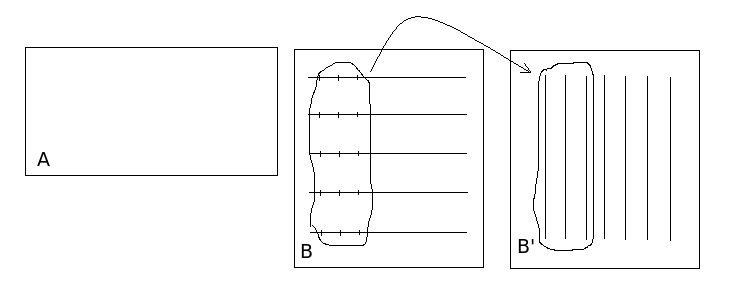
\includegraphics[width=14cm]{B_change.png}
\centering
\label{fig:b_change}
\caption{change in B.}
\end{figure}

\section{Part 1: matrix multiplication: parallel}

Due to the implementation of part 1, i.e. the multiplication by blocks, the parallelization of the code turned out being simple.

The only "problems" that emerged were in matching processes and cells in the 2D grid, and also in using MPI\_Recv in some cases.



\end{document}